%! Author = mddzi
%! Date = 02.06.2024

% Preamble
\documentclass[12pt,a4paper,twoside]{report}

% Packages
\usepackage{amsmath}
\usepackage[T1]{fontenc}
\usepackage[utf8]{inputenc}
\usepackage{lmodern}
\usepackage{textcomp}
\usepackage{lastpage}
\usepackage{geometry}
\usepackage{graphicx}
\usepackage{fancyhdr}
\usepackage[svgnames]{xcolor}
\usepackage[font={small,color=Grey},labelsep=period,width={0.8\textwidth}]{caption}
\usepackage{float}
\usepackage{multirow}
\usepackage{subcaption}
\usepackage{adjustbox}
\usepackage{longtable}
\usepackage{etoolbox}
\usepackage{hyperref}
\usepackage{pdfpages}
\usepackage{indentfirst}
\usepackage{icomma}
\usepackage{natbib}
%\usepackage[backend=bibtex, sorting=none]{biblatex}

\geometry{margin=3.5cm}

\renewcommand{\figurename}{Rysunek}
\renewcommand{\chaptername}{Rozdział}
\renewcommand{\contentsname}{Spis treści}
\renewcommand{\bibname}{Bibliografia}

\pagestyle{fancy}

\title{\textbf{Program do tworzenia schematów układów scalonych w formie gry edukacyjnej}\\[2ex]
    \large Program for creating IC diagrams in the form of an educational game\\
}
\author{Maksymilian Dziemiańczuk}
\date{}

\fancyhf{}
\fancyhead{}
\fancyhead[RO,LE]{Maksymilian Dziemiańczuk}
\fancyhead[RO,LE]{Projekt inżynierski}
\fancyfoot{}
\fancyfoot[RO,LE]{\thepage}
\fancyfoot[RE,LO]{\footnotesize Program do tworzenia schematów układów scalonych w formie gry edukacyjnej}
\fancypagestyle{plain}{
    \renewcommand{\headrulewidth}{0pt}
    \fancyhf{}
    \fancyfoot[RO,LE]{\thepage}
    \fancyfoot[RE,LO]{\footnotesize Program do tworzenia schematów układów scalonych w formie gry edukacyjnej}
}

% Document
\begin{document}

%\maketitle
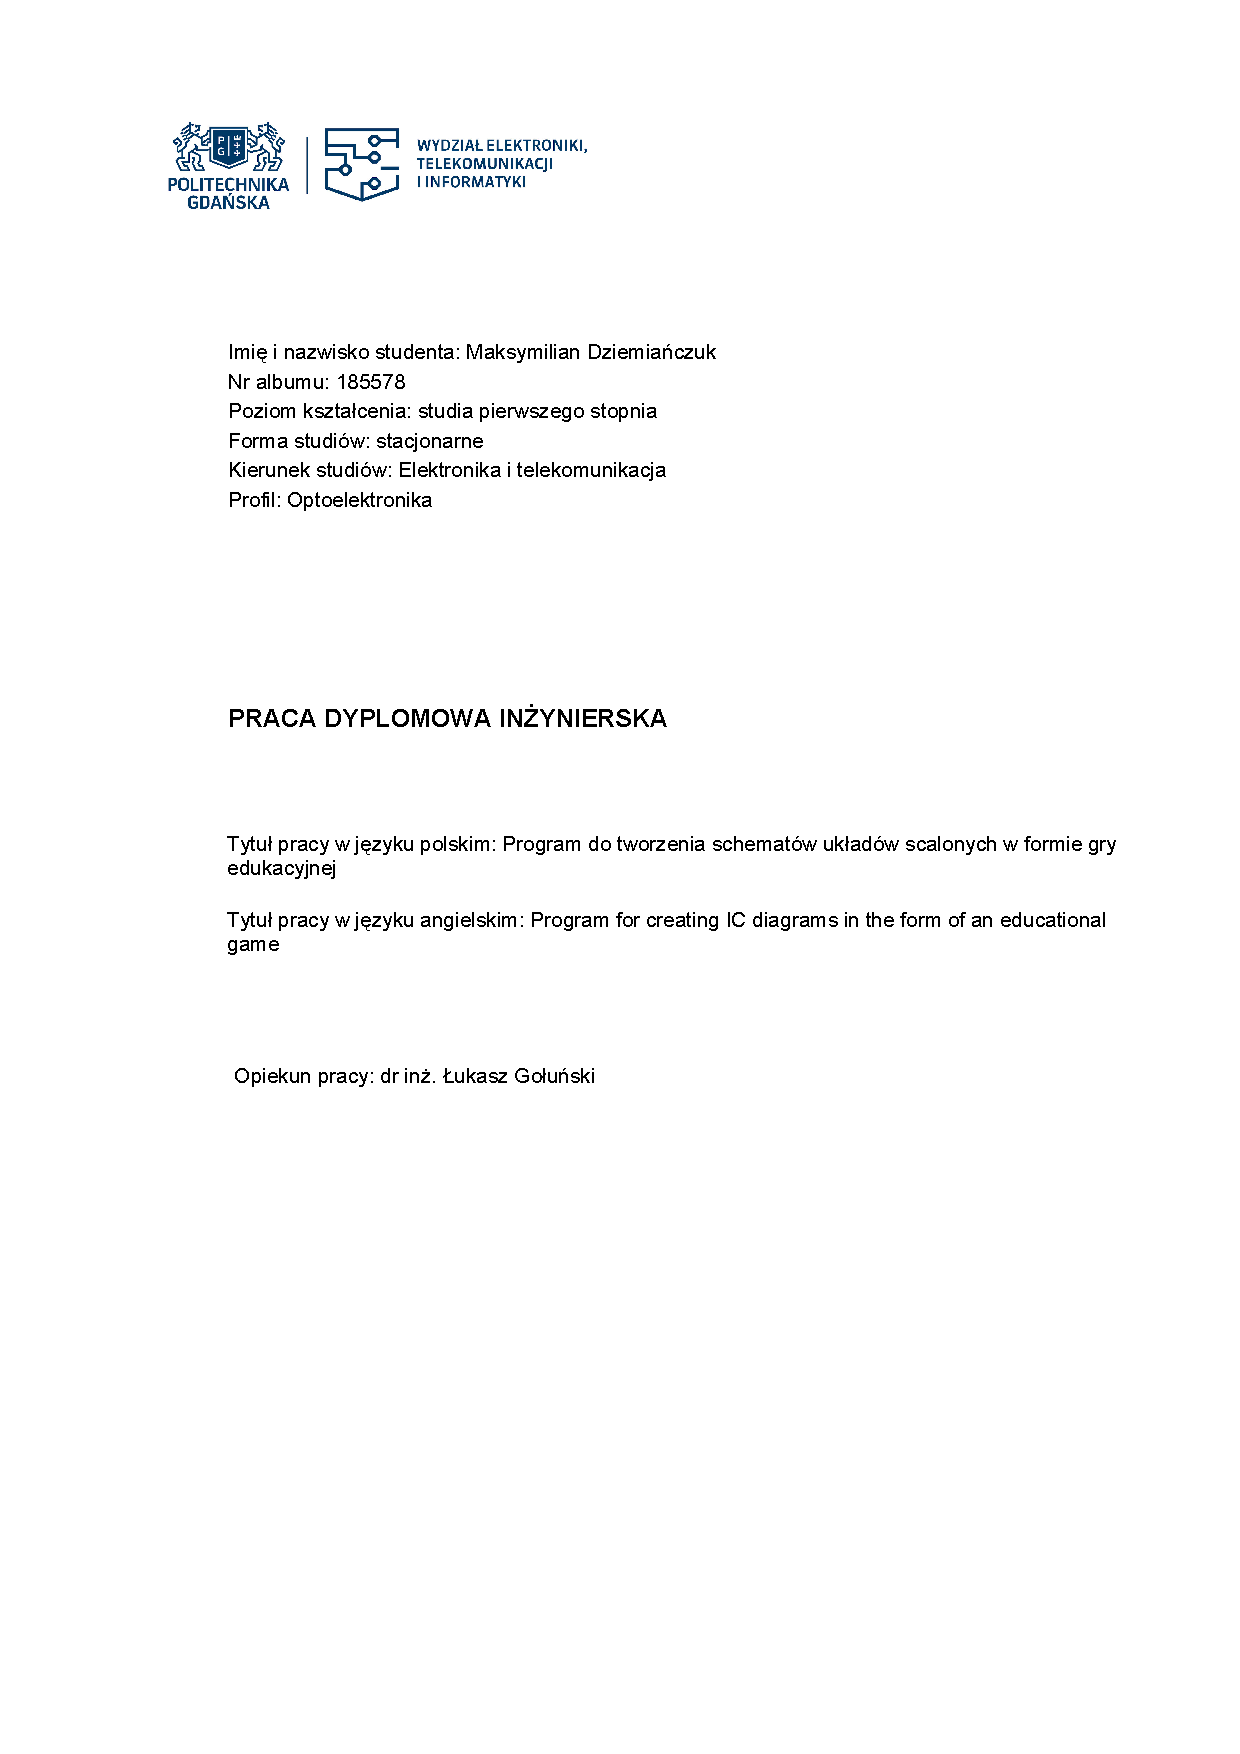
\includepdf[pages={1}]{StronaTytulowa_185578.pdf}

%pusta strona
\newpage \thispagestyle{empty} \ \newpage

\section*{Streszczenie}
\thispagestyle{plain}

Lorem ipsum dolor sit amet, consectetur adipiscing elit

\tableofcontents

\chapter{Wstęp i cel pracy}

Programy do tworzenia schematów są jednym z~kluczowych elementów
procesu wielkoskalowej integracji układów scalonych (ang. VLSI — Very Large Scale Integration)~\cite{VLSI_insemi}.
Polega to na projektowaniu podukładów o określonych funkcjach,
które następnie są łączone w~jeden, w~pełni działający układ scalony.
Taki proces upraszcza projektowanie oraz produkcję układów scalonych, ponieważ prace można podzielić na mniejsze,
mniej skomplikowane części.
Dodatkowo wiele podukładów może być wykorzystywanych w~różnych projektach,
co~znacznie zwiększa efektywność pracy i~obniża jej koszty.
W~efekcie,
programy wspierające projektowanie schematów są nieodzownym narzędziem przy tworzeniu układów scalonych.
%w~ten sposób upraszczany jest proces projektowania oraz produkcji układów scalonych,
%gdyż pracę można podzielić na mniejsze części,
%a~dodatkowo cześć podukładów może być używana w~wielu różnych projektach.
Przykładem takiego programu jest open-source'owy (o publicznym kodzie źródłowym),
Magic VLSI stworzony przez Johna Ousterhouta w~1980 roku,
napisany w~języku C na platformę Linux~\cite{MAGIC_article}.
Charakteryzuje go prosta szata graficzna oraz szeroki zakres działania,
lecz jego obsługa bywa często nieintuicyjna oraz nieprzyjazna dla początkujących użytkowników.
Kolejnym powszechnie dostępnym programem jest Microwind,
na który składa się zestaw modułów,
jednym z~nich jest edytor schematów~\cite{Microwind}.
Niestety, aby używać pełnej i~aktualnej wersji oprogramowania potrzebna jest licencja.
W~wielu innych przypadkach programy te~są~dostępne jedynie w~wersjach płatnych, kierowanych do dużych firm.
To właśnie wysoki próg wejścia
i~złożoność obsługi tego rodzaju programów stały się inspiracją do opracowania tego projektu.\\
%\indent Celem tej pracy było stworzenie
%programu edukacyjnego w~formie gry, który pomoże w~nauce tworzenia schematów układów scalonych,
%ponieważ już same gry komputerowe, nawet te~niemające wyraźnie edukacyjnego charakteru,
%mogą rozwijać umiejętności graczy dzięki stawianiu przed nimi angażujących wyzwań
%i~zachęcaniu do rozwiązywania problemów w kreatywny sposób~\cite{videogames}.\\
\indent Celem tej pracy było opracowanie programu edukacyjnego w~formie gry,
który pomoże w nauce tworzenia schematów układów scalonych.
Gry komputerowe, nawet te~niemające wyraźnie edukacyjnego charakteru,
mogą rozwijać umiejętności graczy.
Osiągają to~poprzez stawianie przed nimi angażujących wyzwań oraz zachęcanie do kreatywnego rozwiązywania problemów~\cite{videogames}.\\
\indent Jedne z~głównych programu założeń to prostota obsługi, intuicyjność oraz ergonomia,
na które mają wpływ przede wszystkim dobrze zaprojektowany interfejs graficzny użytkownika
oraz wbudowane narzędzia wspierające edycję schematu.
%Na tych założeniach opiera się cała część projektu związana z~interfejsem użytkownika.\\
Funkcje te~stanowią podstawę części projektu związaną z~interfejsem użytkownika
i~odpowiadają za poprawę użyteczności
oraz dostępność aplikacji.\\
\indent Kolejnym istotnym elementem tej pracy było przygotowanie angażującej
i~skalowalnej pętli rozgrywki,
która pozwoli na stopniowe wprowadzanie użytkownika w~proces projektowania schematów układów scalonych,
wraz z~implementacją systemów sprawdzania poprawności wykonanych zadań, wskazywania błędów i~ewentualnych podpowiedzi.
%Dzięki realizacji założeń program pomoże w~nauce podstaw bez odrzucania użytkownika
%przez zbyt skomplikowaną obsługę.\\
Dzięki realizacji założeń, projekt ten pozwoli użytkownikowi na zdobycie podstawowej wiedzy
i~umiejętności z~zakresu projektowania układów scalonych,
bez konieczności przechodzenia przez trudniejsze w~obsłudze, tradycyjne oprogramowanie.\\
\indent Zważając na wszystkie założenia oraz charakter edukacyjno-growy projektu,
do realizacji wybrano silnik Unity Engine,
bazujący na języku C\#,
powszechnie wykorzystywany w~tworzenia gier komputerowych.
%program został stworzony w~silniku Unity Engine,
%powszechnie używanym do tworzenia gier komputerowych.
%natomiast możliwość łatwego tworzenia interaktywnej aplikacji graficznej sprawdzi się w~tego typu zastosowaniach.\\
Wybór Unity podyktowany był prostotą tworzenia aplikacji graficznych oraz łatwego tworzenia interaktywnych elementów,
co~można wykorzystać nie tylko w~grach, ale również w~różnego typu narzędziach.
Dzięki Unity,
program łączy funkcje gry z~elementami edukacyjnymi,
tworząc przystępną i~atrakcyjną platformę do nauki podstaw projektowania układów scalonych.
%Został on wybrany ze względu na prostotę tworzenie aplikacji graficznych oraz łatwego tworzenia interaktywnych elementów,
%coi~można wykorzystać nie tylko w~grach, ale również w~różnego typu narzędziach.
%Aby ujednolicić schematy oraz zadania do wykonania dla użytkowników,
%projektowanie będzie odbywać się w~tylko jednej technologii\ \textendash \ CMOS AMIS ami-C5.
%Powodem wyboru tej technologii jest wcześniejsze doświadczenie w~projektowaniu schematów układów scalonych
%w~tej technologii.


%\LaTeX{} \cite{VLSI} is a set of macros built atop \TeX{} \cite{texbook}.

\bibliography{main}
\bibliographystyle{unsrt}

\end{document}
